% ═══════════════════════════════════════════════════════════════════════
%  Section 3 — System Architecture
% ═══════════════════════════════════════════════════════════════════════

\section{System Architecture and Technology Stack}
\label{sec:architecture}

With the requirements defined, this section explains the architectural decisions that shape how Meridian is built and deployed.

\subsection{Technology Choices}

Each technology was chosen to serve a specific security or development need:

\begin{itemize}
    \item \textbf{FastAPI (Python)} — Provides native async support, automatic OpenAPI documentation, and — critically — Pydantic schema validation that rejects malformed input before it reaches business logic. Its dependency injection system cleanly separates authentication from route handlers.
    \item \textbf{React 18 + Vite} — Component-based architecture for reusable UI elements. JSX automatically escapes variables, providing built-in XSS protection on the client side.
    \item \textbf{PostgreSQL 16} — ACID-compliant with native UUID columns, JSONB for flexible audit log details, and robust access control. Parameterized queries via SQLAlchemy eliminate SQL injection.
    \item \textbf{Nginx} — Serves as a reverse proxy with TLS termination, adding security headers and rate limiting at the edge.
    \item \textbf{Docker + GitHub Actions} — Containerized builds ensure environment consistency. CI/CD pipelines automate linting, testing, and image publishing.
\end{itemize}

\subsection{System Layout}

The platform follows a three-tier architecture. The React frontend communicates with the FastAPI backend over HTTPS, which in turn interacts with PostgreSQL for structured data and an encrypted filesystem for resume storage.

\begin{center}
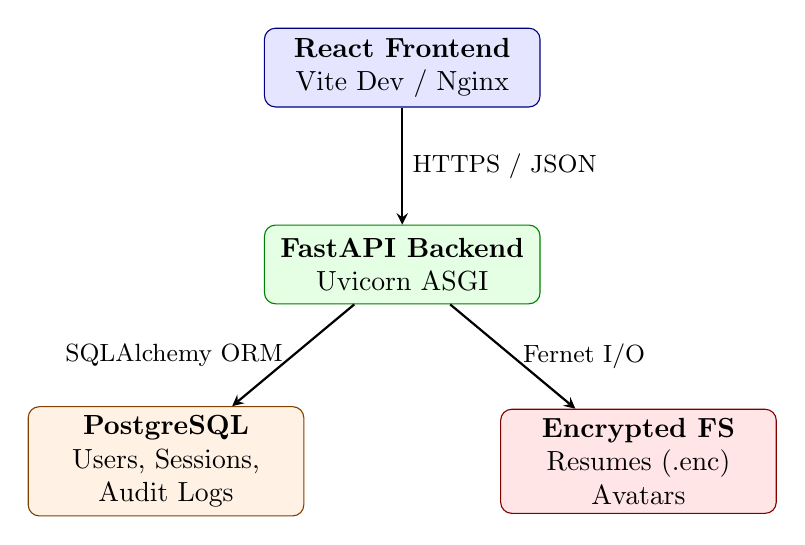
\begin{tikzpicture}[
    box/.style={draw, rounded corners, minimum width=3.5cm, minimum height=1cm, align=center, fill=#1!10, draw=#1!50!black},
    arrow/.style={->, thick, >=stealth}
]
    \node[box=blue] (client) at (0, 6) {\textbf{React Frontend}\\Vite Dev / Nginx};
    \node[box=green] (api) at (0, 3.5) {\textbf{FastAPI Backend}\\Uvicorn ASGI};
    \node[box=orange] (db) at (-3, 1) {\textbf{PostgreSQL}\\Users, Sessions,\\Audit Logs};
    \node[box=red] (fs) at (3, 1) {\textbf{Encrypted FS}\\Resumes (.enc)\\Avatars};
    \draw[arrow] (client) -- node[right, font=\small] {HTTPS / JSON} (api);
    \draw[arrow] (api) -- node[left, font=\small] {SQLAlchemy ORM} (db);
    \draw[arrow] (api) -- node[right, font=\small] {Fernet I/O} (fs);
\end{tikzpicture}
\end{center}

\subsection{Backend Organization}

The backend follows a clean separation of concerns. Each module has a single responsibility, and dependencies flow downward:

\begin{itemize}
    \item \texttt{routers/} — HTTP endpoint handlers, one file per feature (auth, users, resumes, admin, profile)
    \item \texttt{models/} — SQLAlchemy ORM models that define the database schema
    \item \texttt{schemas/} — Pydantic models that validate and sanitize all incoming data
    \item \texttt{security/} — Cryptographic primitives: password hashing, JWT issuance, TOTP, file encryption, CSRF tokens
    \item \texttt{dependencies.py} — Reusable authentication and RBAC checks injected via \texttt{Depends()}
\end{itemize}

This structure means a router never directly touches the database schema definition, and security primitives are never scattered across route handlers — they live in one auditable place.

\subsection{Database Design}

The database schema centers around the \texttt{users} table, with related tables for sessions, resumes, audit logs, and profile data:

\begin{table}[H]
\centering
\small
\begin{tabular}{p{3cm} p{10cm}}
    \toprule
    \textbf{Table} & \textbf{Purpose} \\
    \midrule
    \texttt{users} & Core accounts: Argon2id hash, Fernet-encrypted TOTP secret, role, suspension flag \\
    \texttt{sessions} & JWT tracking: refresh token JTI, device fingerprint, revocation status, expiry \\
    \texttt{resumes} & Metadata only (filename, path, size) — actual content is encrypted on disk \\
    \texttt{audit\_logs} & Immutable event log: action type, actor, IP, timestamp, JSONB detail payload \\
    \texttt{used\_otps} & TOTP replay prevention: stores used codes with their time-step window \\
    \bottomrule
\end{tabular}
\end{table}

\subsection{CI/CD Pipeline}

Every push to \texttt{main} triggers a two-stage pipeline:

\begin{enumerate}
    \item \textbf{CI} — Runs \texttt{ruff} (Python linter) and \texttt{ESLint} (JS linter), then builds the frontend to verify no compilation errors.
    \item \textbf{CD} — Builds Docker images for both backend and frontend, tags them with the commit SHA, and pushes to GitHub Container Registry.
\end{enumerate}

This ensures that broken code never reaches the deployment stage, and every deployed image is traceable to a specific commit.
